% !TEX root = slides.tex
%=========================
\begin{frame}[t]
\label{issues}
\frametitle{\large{Explicit model discrepancy: issues for physical models}}

\centerline{
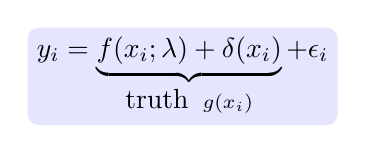
\begin{tikzpicture} \node [rounded corners,fill=blue!10] {
$y_i=\underbrace{f(x_i;\lambda)+\delta(x_i)}_{\textrm{truth  } \: g(x_i)}+\epsilon_i$
};
\end{tikzpicture}
}

%\centerline{\qquad data model: \hfill
%\begin{tikzpicture} \node [rounded corners,fill=blue!20] {
%$y_i=f(x_i;\lambda)+\delta(x_i)+\eid$
%};
%\end{tikzpicture}
%\hspace*{14mm}
%}
%\medskip
%\centerline{\qquad calibrated predictive model: \hfill
%\begin{tikzpicture} \node [rounded corners,fill=blue!20] {
%$y_{mod}(x)=f(x;\lambda)+\delta(x)$
%};
%\end{tikzpicture}
%\hfill
%}

\small

\bbi
\setlength{\itemsep}{2.5mm}
\setlength{\itemindent}{-2.5mm}
\item Explicit additive statistical model for model error $\delta(x)$ \color{blue}\tiny[Kennedy-O'Hagan, 2001]\color{black}
\small
\medskip
\item Potential violation of physical constraints
%\bgi
%\item  \eg incompressible flow: $\nabla\pdot v=0$
%\egi
\item Disambiguation of model error $\delta(x_i)$ and data error $\epsilon_i$
\item Calibration of model error on measured observable does not
      impact the quality of model predictions on other QoIs
      \item Physical scientists are unlikely to augment their model with a statistical model error term on select outputs
      \bri
      \item Calibrated predictive model: $\quad f(x;\lambda)+\delta(x)\:$ or $\: f(x;\lambda)$ ?
      \eri
      \item Problem is highlighted in model-to-model calibration ($\epsilon_i=0$)
\bri
\item no a priori knowledge of the statistical structure of $\delta(x)$
\eri

\ebi


\end{frame}




% \begin{frame}[t]
% \label{merr:3}
% \frametitle{Model Error -- Challenges with current methods}
% \vspace*{0mm}


% \hspace*{1cm}
% \parbox{0.4\textwidth}{$\qquad\textrm{Total error budget}$\\

% \begin{tikzpicture} \node [rounded corners,fill=blue!20] {
% $y_i=\underbrace{f(x_i;\lambda)+\delta(x_i)}_{\textrm{Truth }g(x_i)}+\epsilon_i$
% };
% \end{tikzpicture}
% }
% \begin{tabular}{ p{0.3\textwidth}  p{0.27\textwidth}  }
% \includegraphics[height=0.35\textheight,clip]{merr/test_sketch/{data_fit_model_50_abc}.eps}
% \end{tabular}

% %\small
% \medskip
% \setlength{\leftmargini}{14pt}
% \bi
%  \setlength{\itemsep}{3mm}
% \item Ignoring model error $\delta(x)$ leads to incorrect predictive errors
% \item Conventional statistical modeling (Kennedy and O'Hagan, 2001)
% \bi
% \item makes it difficult to disambiguate model/data errors
% \item may violate physical constraints
% \item not meaningful for prediction of other QoIs
% \ei

% \item Issue is highlighted in model-to-model calibration ($\epsilon_i=0$)
% \bi
% \item no a priori knowledge of the statistical structure of the discrepancy
% \ei
% \ei

% \end{frame}